In order to understand the complexity of the problem \todo{justification for
    modelling with elastic waves} and the
utilised solving method, it is reasonable to revisit some fundamental concepts
in the following chapter. At the same time, a consistent notation is
introduced. At first, the tensor formalism for elastic properties
of rigid bodies is introduced. After that, elastic waves are derived and
analysed further. This discussion will be mostly based on \cite{GrossMarx2014},
if not otherwise stated.
\todo{check if description still applies, citation?}

It should be noted in advance, that vectors are
denoted by a single underline and tensors or
tensor fields of higher order by a number of underlines corresponding to their
order. Also, Einstein summation convention should be applied if no explicit
summation is given in the same formula.

\section{Elastic Properties of Materials}
In the following, the formalism for bulk elastic properties of materials is
introduced. As only small deformations are relevant for the considerations in
this thesis, they are assumed to be in the regime of linear elastic behaviour,
thus neglecting plastic or nonlinear behaviour.

In one dimension linear elastic behaviour can be described simply
by Hooke`s law, which states that a small displacement $\Delta l$ caused by a
force $F$ is proportional to the force.
Considering an object of length $l$ and cross-sectional area $A$,
\textbf{stress} and \textbf{strain} can be defined as

\begin{align}
     & \text{Stress} \quad \quad \sigma := \frac{F}{A}
     & \text{Strain} \quad \quad \epsilon := \frac{\Delta l}{l}
\end{align}.

Hooke`s law can now be reformulated as
\begin{equation}
    \label{eq:HookStress1D}
    \sigma = C\ \epsilon
\end{equation}
with \textbf{Young`s Modulus C} as proportional constant.

\subsection{Stress Tensor}
For objects of finite size, stress can be defined locally on
infinitesimal, cubic volume elements. These volume elements get deformed by
forces that are applied to the object. If we consider a general force
$\Delta \underline{F}$ acting on a surface element $\Delta A$ we can always
divide
this force into a normal component $\Delta \underline{F}_n$ and two mutually
perpendicular tangential components $\Delta \underline{F}_{t1}$ and
$\Delta \underline{F}_{t2}$. This implies the general definition of the stress
tensor
as
\begin{equation}
    \sigma_{ij} = \frac{\text{force in direction i}}{\text{surface with normal
            in direction j}}
\end{equation}
\todo{picture of stress definition?}
where indices i and j denote denote one of the spatial directions x,y or z.
If we assume the volume element to be in equilibrium, it follows that the
normal forces on opposite sites and tangential forces on neighbouring sides
equal each other.
The latter implies that $\sigma_{ij}=\sigma_{ji}$. This leaves 6
independent components, the three normal stresses $\sigma_{ii}$ and the three
shear stresses $\sigma_{ij}$.

\subsection{Strain Tensor}
Deformation of a three-dimensional object can be described using the
displacement field $\underline{u}(\underline{r}, t):=
    \underline{r}^\prime-\underline{r}$,\todo{check definitions}
which defines a displacement vector for each point $\underline{r}$ in space in
comparison to the deformed position $\underline{r}^\prime$. Local stress only
relates to change in displacement relative to neighbouring positions which
allows to consider the Taylor expansion in first order
\begin{equation}
    \underline{u}(\underline{r}+\Delta\underline{r}, t)
    = \underline{u}(\underline{r}, t) +
    \underline{\underline{\gradient}}u(\underline{r}, t)\ \Delta \underline{r}
\end{equation}
with the Jacobian matrix $(\underline{\underline{\gradient}}u )_{ij} =
    \frac{\partial u_i}{\partial r_j}$. This in turn can be decomposed into a
symmetric part and an antisymmetric part. The symmetric part is defined as
strain tensor:
\begin{equation} \label{eq:defstrain}
    \epsilon_{ij} = \frac{1}{2} \left(	 \frac{\partial u_i}{\partial r_j}
    +\frac{\partial u_j}{\partial r_i} \right)
\end{equation}
It is a dimensionless measure for local deformation in contrast to the
antisymmetric part, which represents local rotation.
\todo[color=LightGreen]{why is rotation irrelevant?}

\subsection{Stress-Strain Relations}
Having introduced the stress and the strain tensors, equation
\ref{eq:HookStress1D} can be generalised to three dimensions, thereby taking
anisotropies of the material into account:
\begin{align} \label{eq:HookStress3D}
     & \sigma_{ij} =  C_{ijkl}\epsilon_{kl} \quad\quad\quad
    \quad \quad \text{or}
     & \uuline{\sigma} = \uuline{\uuline{C}} \cdot \uuline{\epsilon}
\end{align}\todo[color=LightGreen]{what is the usual convention?}
This defines the \textbf{Elasticity tensor} as order 4 tensor with unit force
/ area. In general this tensor contains 81 components. However, both the stress

and
the strain tensor are symmetric, so that $C_{ijkl} = C_{jikl} = C_{ijlk}$. This
reduces the number of independent components to 36 and makes it possible to
describe the Elasticity tensor as a $6\cross6$ matrix. For this representation,
the so called Voigt notation maps pairs of coefficients of elasticity, strain
and stress tensor to a single index as in table \ref{tab:voigt}
\begin{table}[t]
    \centering
    \begin{tabular}{cccccc}
        $xx \rightarrow 1$ & $yy \rightarrow 2$    & $zz \rightarrow 3$    &
        $yz=zy
        \rightarrow 4$     & $xz=zx \rightarrow 5$ & $xy=yx \rightarrow 6$
    \end{tabular}
    \caption{Voigt notation}
    \label{tab:voigt}
\end{table}
This simplifies the notation of elasticity significantly, but it should be
treated carefully. Tensors written in Voigt notation do not transform like
vectors in each index.

One can also proove, that $C_{ijkl} = C_{klij}$ considering elastic energy (see
section 4.3.1 of \cite{GrossMarx2014}) which leads to 21 independent
components. Further simplifications derive from crystal symmetry or
limitations in anisotropy. In the following treatment, the material is assumed
to be isotropic, which reduces the number of independent components to 2. These
are typically introduced as Lamé constants $\lambda$ and $\mu$ defined by the
relation
\begin{equation} \label{eq:StressStrainIso_tensor}
    \sigma_{ij} = \lambda \delta_{ij} \epsilon_{kk} + 2\mu \epsilon_{ij}
\end{equation}
\todo{mention of einstein convention?}
which derives from equation \ref{eq:HookStress3D} by regarding isotropy of the
material \cite{kundu2012ultrasonic}. From this equation the elasticity tensor
can be expressed by a simplified $6\cross6$ matrix as in:
\begin{equation} \label{eq:StressStrainIso}
    \uuline{\sigma} = \uuline{\uuline{C}}\cdot \uuline{\epsilon} =
    \begin{pmatrix}
        \lambda + 2\mu & \lambda        & \lambda        & 0    & 0    & 0
        \\
        \lambda        & \lambda + 2\mu & \lambda        & 0    & 0    & 0
        \\
        \lambda        & \lambda        & \lambda + 2\mu & 0    & 0    & 0
        \\
        0              & 0              & 0              & 2\mu & 0    & 0
        \\
        0              & 0              & 0              & 0    & 2\mu & 0
        \\
        0              & 0              & 0              & 0    & 0    & 2\mu
        \\
    \end{pmatrix}
    \cdot
    \begin{pmatrix}
        \epsilon_1 \\ \epsilon_2 \\ \epsilon_3 \\ \epsilon_4 \\ \epsilon_5 \\
        \epsilon_6 \\
    \end{pmatrix}
\end{equation}

\section{Elastic Waves}
This formalism can now be used to introduce elastic waves. Their existence and
behaviour depends on the equations of motion of the regarded medium. To obtain
these, we consider at first a small volume $\Delta V = \Delta x \Delta y
    \Delta z$ that is subject to a stress $\sigma_{xx}(x)$ on the one side and
to $\sigma_{xx}(x+\Delta x)$ on the other side. The resulting net force becomes
thus
\begin{equation}
    \Delta F_x = \left[ \sigma_{xx}(x+\Delta x)- \sigma_{xx}(x) \right] \Delta
    z \Delta y = \diff{\sigma_{xx}}{x} \Delta x \Delta y \Delta z
\end{equation}
by approximating $\sigma_{xx}(x+\Delta x)$ in first order and setting the frame
of reference to the center of mass of the volume.
The force leads to a displacement $u_x$ of the volume in x direction and equals
the
product of the mass $\rho\Delta x \Delta y \Delta z$ and acceleration in x
direction $\ddiff{u_x}{t}$. This yields the one dimensional partial
differential equation
\begin{equation}
    \rho \ddiff{u_x}{t} = \diff{\sigma_{xx}}{x}
\end{equation}
Assuming an isotropic material and using relation \ref{eq:HookStress3D} we
get
\begin{equation}
    \rho \ddiff{u_x}{t} = C_{11} \diff{\epsilon_{xx}}{x} = C_{11}\ddiff{u_x}{x}
\end{equation}
In an anisotropic medium the other stress components need to be taken into
account leading to the general wave equation
\begin{equation} \label{eq:wave_eq}
    \rho \ddiff{u_i}{t} = \diff{\sigma_{ij}}{x_j} = C_{ijkl}
    \Ddiff{u_l}{x_j}{x_k}
\end{equation}
% In analogy to electromagnetic waves we can now make the harmonic plane wave
% ansatz $\uline{u}(\uline{x}, t)= \uline{u}_0\ e^{i(\uline{k}\uline{x}-\omega
%             t)}$. At this, the vector $\uline{k}=\frac{2\pi}{\lambda}$ denotes
% the wave vector defined over the wavelength $\lambda$. $\omega$ is the circular
% frequency defined over the  oscillation frequency $f$ with  $\omega = 2 \pi f$.

% As this solution can be understood as a single frequency mode in Fourier
% transformation, one can achieve arbitrary wave shapes by transforming a mode
% distribution $\uline{u}_0 = \uline{u}_0(\uline{k})$ via Fourier transformation.
% Such an arbitrary wave will behave according to the behaviour of
% the individual plane waves which will be discussed in the following.

% In case of an anisotropic medium one would proceed by substituting the ansatz
% into equation \ref{eq:wave_eq} and

\subsection{Solution for Isotropic Materials}
\label{sec:IsoSolution}
In the following analysis, only isotropic media will be considered. In this
case the isotropic stress-strain relation, equation
\ref{eq:StressStrainIso}, can be inserted in the wave equation which
yields
\begin{equation}
    \rho \ddiff{\uline{u}}{t} = (\lambda + \mu)\ \uline{\gradient}
    (\uline{\gradient}\cdot \uline{u}) + \mu\ \uline{\gradient}^2 \uline{u}
\end{equation}
By using the relation $\gradient^2 \uline u = \uline{\gradient}
    (\uline{\gradient}\cdot \uline{u}) - \uline{\gradient}
    \cross(\uline{\gradient} \cross \uline{u})$ for the vector Laplace operator
one can express it as
\begin{equation} \label{eq:balanceIso}
    \rho \ddiff{\uline{u}}{t} = (\lambda + 2\mu)\ \uline{\gradient}
    (\uline{\gradient}\cdot \uline{u})- \mu\ \uline{\grad }
    \cross (\uline{\gradient}\cross \uline{u})
\end{equation}
If we now consider the Helmholtz decomposition of the displacement fields
\begin{equation} \label{eq:Helmholtz}
    \uline{u} = \uline{\gradient}\Phi + \uline{\gradient}\cross \uline{\Psi}
\end{equation}
with elastic potentials $\Phi$ and $\Psi$ and insert it into
\ref{eq:balanceIso},
it decouples to the two equations (see \cite{BedfordElasticWaves})
\begin{align}
    \ddiff{\Phi}{t} = c_L^2\
     & \uline{\gradient}^2\Phi         \\
    \ddiff{\uline{\Psi}}{t} = c_T^2\
     & \uline{\gradient}^2\uline{\Psi} \\[5pt]
    \text{with } c_L = \left(\frac{\lambda + 2\mu}{\rho}\right)^{1/2} \quad
     &
    \text{ and } \quad c_T = \left(\frac{\mu}{\rho}\right)^{1/2}
    \label{eq:veldef}
\end{align}
Those equations represent four wave equations for the elastic potentials with
phase velocities $c_L$ and $c_T$.

In analogy to electromagnetic waves we can now make the harmonic
plane wave ansatz $\Phi(\uline{x}, t)= u_L\
    e^{i(\uline{k}_L \uline{x}-\omega t)}$ and $\uline{\Psi}(\uline{x}, t)
    =
    \uline{u}_T \ e^{i(\uline{k}_T\uline{x}-\omega t)}$ with arbitrary
amplitudes $u_L\in\mathbb{C}$ and $\uline{u}_T\in \mathbb{C}^3$.
Here, the vector
$\uline{k}=\frac{2\pi}{\lambda}$ denotes the wave vector defined by the
wavelength $\lambda$ and $\omega$ is the circular frequency defined by the
oscillation frequency $f$ with	$\omega = 2 \pi f$. The differentiation between
$\uline{k}_L$ and $\uline{k}_T$ is necessary because of the different
phase velocities for the elastic potentials resulting in different wave numbers
according to $c = \frac{\omega}{|\uline{k}|}$.

Substituting the wave ansätze into equation \ref{eq:Helmholtz}, we get
\begin{equation}
    \uline{u} = u_L \uline{k}\	e^{i(\uline{k}_L\uline{x}-\omega t)}
    + \uline{k} \cross \uline{u}_T\ e^{i(\uline{k}_T\uline{x}-\omega t)}
\end{equation}
Here we can see now, that the elastic potential $\Phi$ is responsible for waves
with longitudinal polarisation and $\uline{\Psi}$ for waves with transversal
propagation. Furthermore we can identify an orthonormal polarisation basis
depending on the propagation direction $\uline{\hat{k}} =
    \frac{\uline{k}}{|\uline{k}|}$ so that $\uline{u}$ decomposes to
\begin{equation} \label{eq:wave_ansatz}
    \uline{u} = a_L \ \uline{p}_L\	e^{i(\uline{k}_L\uline{x}-\omega
            t)}
    + (a_{TH}\ \uline{p}_{TH} + a_{TV}\ \uline{p}_{TV})\
    e^{i(\uline{k}_T\uline{x}-\omega t)}
\end{equation}
In general, the polarisation vector for longitudinal polarisation
$\uline{p}_L$ is fixed to be $\uline{\vec{k}}$. If scattering at an interface
is considered, a plane of incidence can be defined that is spanned by
$\uline{\hat{k}}$ and the normal vector of the interface. The transversal
polarisation vectors are then defined as transversal horizontal polarisation
$\uline{p}_{TH}$ pointing out of the plane of incidence and transversal
vertical polarisation $\uline{p}_{TH}$ lying in plane of incidence orthonormal
to $\uline{\hat{k}}$, here now defined as
$\uline{p}_{TV}=\uline{p}_L \cross \uline{p}_{TH}$.
\todo[color=LightGreen]{decomposition: e.g
    $a_L= \uline{u}(\uline{x}, t)\cdot\hat{k} * e^{-ikx+i\omega t}$ \\?}
\todo{sketch}

To sum up, those polarisation vectors define three polarisation modes L, TH and
TV denoting longitudinal, transveral horizontal and transversal vertical
polarisation which can be superimposed arbitrarily. The coefficients $a_i$ may
be complex to express an additional phase between the components. However, it
should be noted, that this is merely convenient for
calculation and that the physical wave behaves like the real part of the shown
equations.

% \section{Elastic Waves in Stratified Media}
% The previous considerations enable now to target the description of elastic
% wave propagation through layer structures, for instance distributed bragg
% reflectors. Those structures consist of homogeneous materials with different
% mechanical properties and thus phase velocities per material. 
% In the following the layers
% are assumed to be parallel to the xy-plane and have a defined thickness in
% z-direction. In x and y-direction they are infinitely stretched out, which is a
% good approximation, if the thickness is small compared to the width.
% % 
% \todo{alternative: reflecting boundaries on the side}
% % 

\subsection{Elastic Wave Scattering at an Interface}
%Zwischentext einfügen ! #################################################################

\subsubsection{Boundary Conditions}
On the way to describe wave propagation through complex layer structures it is
useful to consider a single interface first. In the upper half space $S_1$ and
lower half space $S_2$
we assume homogeneous materials with different elastic constants and thus
different sound velocities. At the interface, which is chosen to be the
xy-plane the elastic properties are discontinuous. However, we can assume that
those layers connected strongly so that the displacement field and normal
stresses are continuous at the boundary \cite[182,185]{achenbach1973wave}. This
leads to the boundary conditions:
\begin{align} \label{eq:boundaryconditions}
    \uline{u}^{(1)}(\uline{r}, t)|_{\uline{r}\in\partial S_1}   & =
    \uline{u}^{(2)}(\uline{r}, t)|_{\uline{r}\in\partial S_2}       \\[5pt]
    \sigma_{13}^{(1)}(\uline{r}, t)|_{\uline{r}\in\partial S_1} & =
    \sigma_{13}^{(2)}(\uline{r}, t)|_{\uline{r}\in\partial S_2}     \\[5pt]
    \sigma_{23}^{(1)}(\uline{r}, t)|_{\uline{r}\in\partial S_1} & =
    \sigma_{23}^{(2)}(\uline{r}, t)|_{\uline{r}\in\partial S_2}     \\[5pt]
    \sigma_{33}^{(1)}(\uline{r}, t)|_{\uline{r}\in\partial S_1} & =
    \sigma_{33}^{(2)}(\uline{r}, t)|_{\uline{r}\in\partial S_2}
\end{align}
In these six equations displacement and stress from upper and lower medium are
differentiated by the given superscript index.

\subsubsection{Law of Refraction} \label{sec:lawofrefr}
% spatial orientation
If we now consider a plane wave\todo[color=LightGreen]{introduced in 2.2.1}
that is incident on that interface, we can define a plane of incidence as in
section \ref{sec:IsoSolution} and rotate the
coordinate system so that it equals the yz-plane which simplifies the
polarisation basis. This leaves the physical problem only invariant, if we
assume an isotropic material as stated before.
In that setting, the wave vector $\uline{k}_i$ for a particular mode $i \in
    \{L,TV,TH\}$ can be parametrised by the angle of incidence $\theta$ as
\todo{consistent mode description}
\begin{equation} \label{eq:k_fromangle}
    \uline{k}_i = \frac{\omega}{c_i}\, ( 0,\ \sin(\theta_i),\ -\cos(\theta_i)\
    )^T
\end{equation}
% polarisation basis
The polarisation basis can then be defined as
\begin{align}
    \uline{p}_L = \uline{\hat{k}} & = ( 0,\ \sin(\theta_i),\ -\cos(\theta_i)\
    )^T
    \\
    \uline{p}_{TH}                & = (\ 1,\ 0,\ 0)^T
    \\
    \uline{p}_{TV}                & = \uline{p}_L \cross \uline{p}_{TH}
    = ( 0,\ -\cos(\theta), -\sin(\theta))^T
\end{align}
% general snellius
It is now possible to extract a law of refraction from the boundary conditions
in equation \ref{eq:boundaryconditions} (see \cite[168ff]{achenbach1973wave}).
A simple approach is to consider
scattering of the transversal horizontal mode (TH) so that the displacement is
only in x-direction. An incoming plane wave with
wave vector $\uline{k}_{in}$ is partially reflected to a wave along
$\uline{k}_r$ and partially transmitted through the interface to a wave with
$\uline{k}_t$. Also, different frequencies $\omega_i$ are assumed for the
scattered waves so that the wave in the upper medium is
\begin{equation}
    u_1^{(1)} = a_{in}\
    e^{i( k_{in}\sin\theta_{in} y-\omega_{in} t)}
    + a_r\ e^{i( k_{r}(\sin\theta_{r} y -\omega_{r} t)}
\end{equation}
and in the lower medium
\begin{equation}
    u_1^{(2)} = a_{t}\
    e^{i(( k_{t}\sin\theta_{t} y -\omega_{t} t)}
\end{equation}
Here it was used, that the interface is at $z=0$ which simplifies the following
derivation.
According to the boundary conditions, these displacements must equal each other
at any time and for all points on the interface. This leads to the immediate
conclusion, that
\begin{equation} \label{eq:equalfreq}
    \omega = \omega_{in} = \omega_r = \omega_t
\end{equation}
After removing the common factor $e^{-i\omega t}$ from the equation and
expressing the wave numbers by frequency and sound velocity as
$k = \frac{\omega}{c}$, we get
\begin{equation} \label{eq:snelliuscompare}
    a_{in}\ e^{i \frac{ \omega}{c_{T,1}}\sin\theta_{in} y}
    + a_{r}\ e^{i \frac{ \omega}{c_{T,1}}\sin\theta_{r} y}
    = a_{t}\ e^{i \frac{ \omega}{c_{T,2}}\sin\theta_{t} y}
\end{equation}
This however can be only fulfilled for all $y \in \mathbb{R}$ if the relations
\begin{align}
    a_{in} + a_r                      & = a_t                            \\
    \frac{\sin\theta_{in}}{c_{T,1}} = & \frac{\sin\theta_{r}}{c_{T,1}} =
    \frac{\sin\theta_{t}}{c_{T,2}} \label{eq:gensnell}
\end{align}
are met. Equation \ref{eq:gensnell} can be also interpreted as the equality
of the wave vector component parallel to the interface
$k_y=\sin\theta_i \frac{\omega}{c_i}$.

The same procedure can be applied to the y and z component of the displacement
field, where transversal vertical ($TV$) and longitudinal ($L$) modes need to
be considered \cite[185]{achenbach1973wave}. However, one significant
difference is that even for a single incident mode, both $L$ and $TV$ mode are
possible after being reflected or transmitted. This will only add a term of the
form $ a_{i}\ e^{i \frac{ \omega}{c}\sin\theta_{i} y}$ to each side of equation
\ref{eq:snelliuscompare}, but will result in analogous relations to
\ref{eq:equalfreq} and \ref{eq:gensnell}, namely the invariance of frequency
$\omega$ and $k_2$ of each mode under scattering at the interface.

To conclude, the angle $\theta_{out}$ of any outgoing polarisation mode can be
determined from the incoming wave`s angle $\theta_{in}$ and the sound
velocities for incoming and outgoing wave $c_{in}, c_{out}$ by
\begin{equation} \label{eq:generalsnell}
    \frac{\sin\theta_{in}}{c_{in}} =  \frac{\sin\theta_{out}}{c_{out}}
\end{equation}
This can be transferred to the optical law of snellius by introducing an
effective refraction index $n_i = \frac{1}{c_i}$. Consequently, TH-polarised
waves scatter like electromagnetic waves and for example the reflected angle is
always the incident angle.
The main difference to optics becomes clear for L and TV polarised waves.
Scattering within the same polarisation mode is the same as for the TH mode,
but now those modes can scatter into each other. Equation \ref{eq:generalsnell}
still applies, but energy is also emitted to additional modes as shown in
figure \ref{fig:angles}.

% possible additional statements:
% - limited set of angles for any combination of layers

It is also possible to get the analytical solutions for refraction of a single
mode at an interface by evaluating the remaining boundary conditions and the
results from continuity of displacement. The results are usually expressed by
defining a reflection coefficient $r_i$ and a transmission coefficient $t_i$
for participating mode $i \in\{L, TH, TV\}$ as
\begin{align}
    r_i := \frac{a_{r,i}}{a_{in,i}} \\
    t_i := \frac{a_{t,i}}{a_{in,i}}
\end{align}
Usually those coefficients have a functional dependency on the incident angle.

% algebraic solution to single interface?
\subsubsection{Total Internal Reflection}
Total internal reflection is known as the phenomenon when a wave is totally
reflected at a boundary for incident angles greater than a critical angle
$\theta_{tot}$. If $c_1$ and $c_2$ are the phase velocities first and second
medium, the outgoing angle
\begin{equation}
    \theta_2 = \arcsin( \frac{c_1}{c_2} \sin(\theta_1)) \quad c_2 < c_1
\end{equation}
has no real solution for $\theta_1 > \theta_{tot} = \arcsin \frac{c_2}{c_1}$.
There is however a complex solution and this resulting complex angle can be
interpreted in the given wave formalism \cite[5]{brekhovskikh2012waves}. This
interpretation also allows to extend the concept to two arbitrary polarisation
modes that the wave can scatter inbetween, regardless of propagation direction.

Considering the case $\theta_1 > \theta_{tot}$, $\theta_2$ can be expressed as
$\theta_2 = \frac{\pi}{2} + i\alpha,\ \alpha\in\mathbb{R}$. Inserting this into
the general wave solution equation \ref{eq:wave_ansatz}, we need to calculate
the wave vector $\uline{k}$ as in equation \ref{eq:k_fromangle}. This results
in
\begin{align}
    k_y & = k \sin\theta_2 = k \cosh\alpha & k_z= k \cos\theta = ik \sinh\alpha
\end{align}
This complex wave vector inserted into the factor $e^{ik_zz}$ results in
$e^{-k\sinh\alpha} z$ which represents an evanescent wave. This type of wave is
attenuated exponentially so that the wave behaves as expected.

In case of frustrated total internal reflection this exponential behaviour
becomes relevant, when another interface is close to the first reflecting
interface. Then it is possible for the usually totally reflected mode to
transmit intensity into a mode of the third medium.

\subsubsection{Conservation of Energy at a Single Interface}
According to \cite[166]{achenbach1973wave} the transmitted time averaged power
per unit area of a transversal elastic wave in a homogeneous medium is
\begin{equation}
    I_L = \frac{1}{2}(\lambda+2\mu)\frac{\omega^2}{c_L}|a_L|^2
\end{equation}
and similarly for a transversal elastic wave of a single polarisation mode
\begin{equation}
    I_T = \frac{1}{2}\mu\frac{\omega^2}{c_T}|a_T|^2
\end{equation}
where $a_T$ is either $a_{TV}$ or $a_{TH}$ depending on the regarded mode. This
quantity is also known as time averaged intensity. By using the definition of
$c_L$ and $c_T$ from equation \ref{eq:veldef} we get the more general relation
\begin{equation} \label{eq:generalIntensity}
    I_p = \frac{\rho\omega^2}{2} |a_p|^2 c_p
\end{equation}
with $p\in \{L,TH, TV\}$ denoting the polarisation mode. It should be noted
that the referred unit area is perpendicular to the direction of propagation.

\begin{figure*}[h]
    \centering
    \begin{subfigure}{0.49\textwidth}
        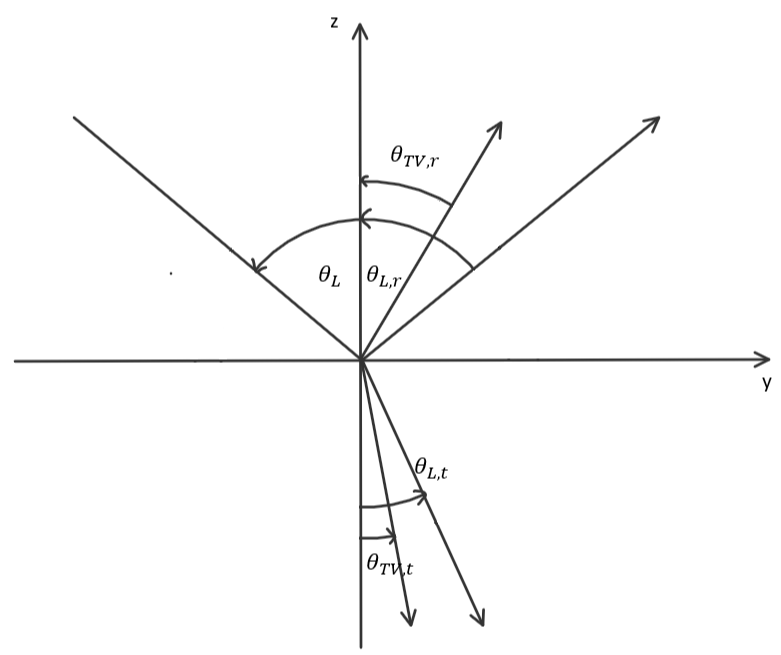
\includegraphics[width=\textwidth]{pictures/L_wave_diffraction.png}
        \caption{Refraction of a Longitudinal Elastic Wave}
        \label{fig:refPwave}
    \end{subfigure}
    \begin{subfigure}{0.49\textwidth}
        \vspace{30pt}
        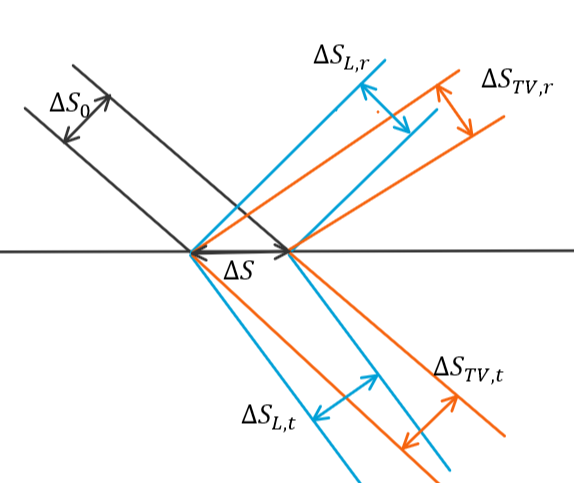
\includegraphics[width=0.8\textwidth]{pictures/energypartition.png}
        \vspace{20pt}
        \caption{Conservation of Energy at Surface Element $\Delta S$ for an TV
            polarized beam}
        \label{fig:energypartition}
    \end{subfigure}
    \caption{}
    \label{fig:angles}
\end{figure*}

In the setting of an arbitrary polarised wave scattered at an interface,
there are six possible outgoing modes as discussed previously.
To get an energy relation between the intensities of each
participating mode we consider the energy balance of a surface element
$\Delta S$ of the interface, on which an arbitrarily polarised beam with
cross-sectional
area $\Delta S_{0}$ and intensity $I_{in}$ is incident. The cross-sectional
areas of the outgoing beams are named according to figure
\ref{fig:energypartition} which can be also transferred to the case of an
incident TH polarised wave.

The power each beam transmits or emits is given by the product $P_p = I_p\
    \Delta S_p$. $\Delta S_p$ is related to $\Delta S$ by $\Delta S_p =
    \cos\theta_p\ \Delta S$,
$p$ denoting any of the depicted beams and $\theta_p$ being the according
angle.

In conclusion, the energy balance results in
\begin{align}
    I_{in} \cos\theta_{in} = \sum\limits_{i=L,TH,TV} I_{i,r}\  \cos\theta_{i,r}
    + I_{i,t}\	\cos\theta_{i,t}
\end{align}

From that we can divide by $I_{in}\cos \theta_{in}$ and define reflectivity
$\mathcal{R}$ and transmittivity $\mathcal{T}$ of the
interface as fraction of reflected and transmitted power by
\begin{align}
    \mathcal{R} := \frac{ I_{L,r}\  \cos\theta_{L,r} + I_{TH,r}
        \cos\theta_{T,r} +
    I_{TV,r}  \cos\theta_{T,r}}{I_{in} \cos\theta_{in}} \\
    \mathcal{T} := \frac{ I_{L,t}\  \cos\theta_{L,t} + I_{TH,t}
        \cos\theta_{T,t} +
        I_{TV,t}  \cos\theta_{T,t}}{I_{in} \cos\theta_{in}}
\end{align}
so that $\mathcal{R} + \mathcal{T} = 1$ is fulfilled. This can be later used to
verify the  obtained results.

\subsection{Scattering at a System of Layers}
The considerations of one interface can now be extended to a system of $N$
interfaces as shown in figure \ref{fig:dbr}. Each layer gets an index $n$
starting from the uppermost layer of index $n=0$. The first interface from the
top is still located at $z_1=0$ and has index $n=1$. The subsequent interfaces
follow below at depths $z_n$. Their depth depends on the intermediate layer
thicknesses $d_n=z_n-z_{n+1}$ with layer index $n$.
Similar as before, we assume now the displacement field in each layer $n$ as
\begin{equation} \label{eq:gendisplacement}
    \uline{u}^{(n)}(\uline{x},t)= \sum\limits_{i\in\{L,TH,TV\}} t_{n,i}
    \uline{p}_{n,i}^t\ e^{i(\uline{k}_{n,i}^t\uline{x} - \omega t)}
    + r_{n,i} \uline{p}_{n,i}^r\ e^{i(\uline{k}_{n,i}^r\uline{x} - \omega t)}
\end{equation} %mention dependency on theta?
This formula is a superposition of a down going wave with quantities denoted by
t and a upgoing wave caused by reflections with quantities denoted by r. The
upgoing $\uline{k}^r$ is flipped in z-direction compared to $\uline{k}^t$.
Further, the complex amplitudes of down and upgoing modes are directly denoted
by $t_{n,i}$ and $r_{n,i}$. As
the angle $\theta_{n,i}$ between $\uline{k}$ and z-axis is changes by
scattering, also $\uline{k}_{n,i}$ and polarisation vector $\uline{p}_{n,i}$ is
different for each material. %genauere beschreibung?
%Angle propagation
%only one incident mode allowed

To evaluate the transmission through the stack of layers, it is the task is now
to calculate the coefficients $t_{N,i}$ and $r_{1,i}$ given coefficients
$t_{1,i}$ and with the assumption $r_{N,i}=0$ for all $i\in\{L,TH,TV\}$.
\todo[color=LightGreen]{correct explanation?}
This assumption can be made because we only consider the incoming power on the
chip. Thermal radiation from the chip itself is significantly lower We
further choose exactly one $t_{1,i}=1$ to mark the incident mode. This
simplifies solving the problem and lets the coefficients $t_{N,i}$ and
$r_{1,i}$ become the transmission and reflection coefficients of the layer
system.

For this, all $6N$ boundary conditions need to be solved. These are constructed
by inserting the general displacement field of each participating layer as in
equation \ref{eq:gendisplacement} in the boundary conditions for a single
interface (equation \ref{eq:boundaryconditions}). As a result each displacement
field of an enclosed layer is evaluated twice, once at the upper boundary and
once at the lower boundary. This results in a phase shift of $e^{-ik_zd_n}$
between upper and lower displacement.

As many systems of equations this problem can be formulated with matrices. In
the following, two solution methods are introduced. In the later course, both
methods will be compared to each other on the base of practical advantages and
disadvantages.

\begin{figure}[h]
    \centering
    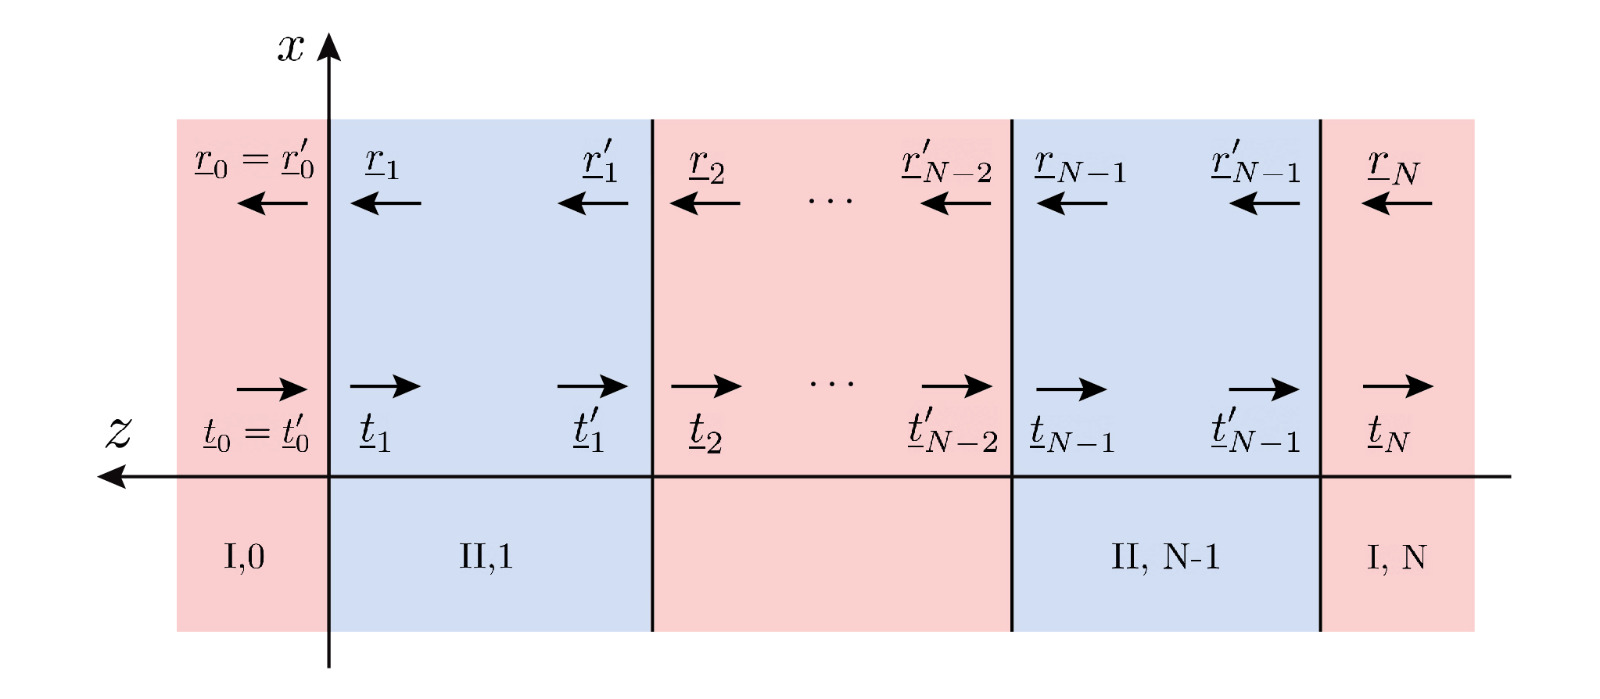
\includegraphics[width=\textwidth]{pictures/DBR_amplitudes_final.jpg}
    \caption{Geometry and amplitude nomenclature of a N layer strong bragg
        reflector}
    \label{fig:dbr}
\end{figure}

\subsubsection{Transfer Matrix Method}
To introduce the matrix formalism of the Transfer Matrix Method (TMM) it is
useful to focus on a single interface with index $n$ between layers $n-1$ and
$n$ located at depth $z_n$. We can define a generalised state vector
$\uline{v}_i$  in each layer $i$ as
\cite{Fomenko2014}
\begin{equation}
    \uline{v}_i = (u^{(i)}_1, u^{(i)}_2, u^{(i)}_3, \sigma^{(i)}_{13},
    \sigma^{(i)}_{23}, \sigma^{(i)}_{33})^T
\end{equation}
Each of the components depends on location $\uline{x}$ and time $t$ in the
layer. We also introduce the superscript "+" for evaluating an arbitrary
multidimensional function of space and layer index $n$ at interface
$\mathcal{F}_n$ and superscript "-" for evaluating at $\mathcal{F}_{n-1}$ so
that the boundary conditions at the n-th interface $\mathcal{F}_n$ are
\begin{equation}
    \uline{v}_n^+ = \uline{v}_{n+1}^-
\end{equation}
In addition to equation \ref{eq:gendisplacement}, the stress components in
$\uline{v}$ can be evaluated as well. From stress strain relation
\ref{eq:HookStress3D} we get for an isotropic material
\begin{align}
    C_{1313}^{(n)}\epsilon_{13}^{(n),+} =                     &
    C_{1313}^{(n+1)}\epsilon_{13}^{(n+1),-}                     \\[5pt]
    C_{2323}^{(n)}\epsilon_{23}^{(n),+} =                     &
    C_{2323}^{(n+1)}\epsilon_{23}^{(n+1),-}                     \\
    \sum\limits_{i=1}^3 C_{33ii}^{(n)}\epsilon_{ii}^{(n),+} = &
    \sum\limits_{i=1}^3 C_{33ii}^{(n+1)}\epsilon_{ii}^{(n+1),+}
\end{align} %possibly change to |_{\uline{r}\in\mathcal{F}_n}
\todo{mention, that propagation of angles is needed first}
Furthermore, the strain can be evaluated by inserting the general displacement
field \ref{eq:gendisplacement} into its definition $\epsilon_{ij} = \frac{1}{2}
    \left( \diff{u_i}{r_j} +\diff{u_j}{r_i} \right)$.

At this point it is neccessary to know all angles at which the different modes
propagate through each layer in order to construct the equations as linear
relations. These can be obtained by following the considerations of section
\ref{sec:lawofrefr}.  Because of our limitation to one incident mode on the top
layer, also only one propagation angle per distinct phase velocity in the
medium is possible. From the structure of
$\uline{u}^{(n)}$ it is possible to construct a $6\cross6$ matrix $M_n$ so that
\begin{equation}
    \uline{v}_n(z) = \uuline{M_n}\ \uuline{P_n}(z-z_n)\uline{a}_n
\end{equation}
The coefficient vector $\uline{a_n}$ of layer $n$ is defined as
\begin{equation}
    \uline{a}_n = (\uline{t}_n, \uline{r}_n)^T	= (t_{n,L}, t_{n,TH}, t_{n,TV},
    r_{n,L}, r_{n,TH}, r_{n,TV})^T
\end{equation}
containing the wave amplitudes at the upper edge of each layer $z = z_n$. As an
exeption, $r_{0,i}$ and $t_{0,i}$ are defined directly at the first interface.

$\uuline{P_n}(z)$ represents the phase factors due to wave propagation
as diagonal matrix
\begin{equation} \label{eq:PmatTMM}
    \uuline{P_n}(z) = \text{diag}\{ e^{ik_{z,n}^{(L)}z},
    e^{ik_{z,n}^{(TH)}z},
    e^{ik_{z,n}^{(TV)}z}, e^{-ik_{z,n}^{(L)}z}, e^{-ik_{z,n}^{(TH)}z},
    e^{-ik_{z,n}^{(TV)}z}\}
\end{equation}
\todo[color=LightGreen]{clear?}
The factor $e^{k_{y,n}^{(i)} y}$ was removed from the expression as it does not
change at the boundary. This automatically sets the phase of the displacement
wave to zero at the upper boundary of the layer. The coefficients at the lower
boundary are in the following denoted by $\uline{a}_n^\prime =
    \uuline{P_n}(-d_n)\ \uline{a}_n$.

As a result the boundary conditions at an individual interface between layers
$n-1$ and $n$ can be written as
\begin{equation}
    \uuline{M}_{n-1}\ \uline{a}_{n-1}^\prime = \uuline{M}_{n}\ \uline{a}_{n}
\end{equation}
If we assume that $\uuline{M}_{n}$ is invertible, we can define the
transfer matrix $S_n$ by
\begin{equation}
    \uline{a}_{n} = \uuline{M}_{n}^{-1}\ \uuline{M}_{n-1}
    \uline{a}_{n-1}^\prime
    = \uuline{S}_n \uline{a}_n^\prime
\end{equation}
which enables us to obtain the wave coefficients after scattering by a simple
matrix multiplication.

With this knowledge we can assemble a global transfer matrix for all interfaces
by
\begin{equation} \label{eq:Scomposition}
    \uuline{S} = \uuline{S}_N\cdot \uuline{P}_{N}(z_{N}-z_{N-1})\cdot
    \uuline{S}_{N-1} \cdot \uuline{P}_{N-1}(z_{N-1}-z_{N-2}) \cdots
    \uuline{S}_2
    \cdot \ \uuline{P}_2(z_{2}-z_{1}) \cdot \uuline{S}_1
\end{equation}
so that the final wave coefficients $\uline{a}_N$ below the lowest interface
are
\begin{equation}
    \begin{pmatrix} \uline{t}_n \\ \uline{r}_n	\end{pmatrix}
    = S\cdot  \begin{pmatrix} \uline{t}_1 \\ \uline{r}_1 \end{pmatrix} =
    \begin{pmatrix}
        \uuline{T} & \uuline{C}_1 \\ \uuline{C}_2 & \uuline{R}
    \end{pmatrix} \cdot \begin{pmatrix} \uline{t}_1 \\ \uline{r}_1
    \end{pmatrix}
\end{equation}
Remembering that $\uline{r_n}=0$, we can solve for $\uline{r}_1$ and
$\uline{t}_n$
\begin{align}
    \uline{r}_1 & = -\uuline{R}^{-1}\ \uuline{C}_2\ \uline{t}_1             \\
    \uline{t}_n & = \begin{pmatrix} \uuline{T},& \uuline{C}_1 \end{pmatrix}
    \cdot \begin{pmatrix} \uline{t}_1 \\ -\uuline{R}^{-1}\ \uuline{C}_2\
              \uline{t}_1\end{pmatrix}
\end{align}
%@appendix:
% exact extraction of matrix elements,
% explain removal of y dependency

\subsubsection{Linear System of Equations}
As an alternative, a more direct solving approach is presented by solving the
system of linear equations with the inversion of a single matrix. This method
will be called from now on LSE-method (Linear System of Equations).

For this method the coefficients for upgoing waves are defined to have their
phase origin at the lower interface instead of the upper interface as defined
in \ref{eq:PmatTMM}, so that the P-matrix becomes
\begin{equation}
    \uuline{P_n}(z) = \text{diag}\{ e^{ik_{z,n}^{(L)}z},
    e^{ik_{z,n}^{(TH)}z},
    e^{ik_{z,n}^{(TV)}z}, e^{-ik_{z,n}^{(L)}(z+d_n)},
    e^{-ik_{z,n}^{(TH)}(z+d_n)},
    e^{-ik_{z,n}^{(TV)}(z+d_n)}\}
\end{equation}.
The reason is that the diagonal entries evaluated at the layer boundaries $z=0$
and $z=-d_n$ will now have always absolute values of $1$ or lower. The latter
is true for total internal reflection in contrary to $\uuline{P}_n$ from TMM.

For better clarity in notation we can rewrite matrix $\uuline{M}_n$ as
composition of two $6\cross 3$ matrices $\uuline{M}_n = (\uuline{T}_n,
    \uuline{R}_n)$ and $\uuline{P}_n$ as block diagonal of two $3\cross 3$
matrices $\uuline{P}_n = \mathit{diag}\{\uuline{D}_n(z),\
    \uuline{D}_n(-(z+d_n))
    \})$. The diagonal matrix $\uuline{D}_n$ is here defined as a $3\cross3$
diagonal matrix with $\uuline{D}_n(z) = \text{diag}\{ e^{ik_{z,n}^{(L)}z},
    e^{ik_{z,n}^{(TH)}z}, e^{ik_{z,n}^{(TV)}z}\}$

The boundary conditions at interface $n$, below layer $n$ are then
\begin{equation}
    \left(\uuline{T}_n,\ \uuline{R}_n\cdot \uuline{D}_n(-d_{n}) \right)
    \begin{pmatrix} \uline{t}_n \\ \uline{r}_n \end{pmatrix} =
    \left( \uuline{T}_{n-1} \cdot \uuline{D}_{n-1}(-d_{n-1}),\
    \uuline{R}_{n-1} \right)
    \begin{pmatrix} \uline{t}_{n-1} \\ \uline{r}_{n-1} \end{pmatrix}
\end{equation}
With $\uuline{T}_{n-1}^\prime = \uuline{T}_{n-1} \cdot
    \uuline{D}_{n-1}(-d_{n-1})$ and analogously for $\uuline{R}_n^\prime$, this
is equivalent to
\begin{equation}
    \left(\uuline{T}_{n-1}^\prime,\ \uuline{R}_{n-1}
    -\uuline{T}_n,\ -\uuline{R}_n^\prime,\right)
    \begin{pmatrix} \uline{t}_{n-1} \\ \uline{r}_{n-1} \\  \uline{t}_n \\
        \uline{r}_n\end{pmatrix} = 0
\end{equation}
This denotes now a $6\cross 12$ matrix for a single interface. In general the
total
system is constructed as $6N \cross 6N$ matrix
\begin{equation}
    \begin{pmatrix}
        \uuline{R}_0         & -\uuline{T}_1           & -\uuline{R}_1^\prime &
        0
                             & 0                       & \cdots               &
        0
        \\
        0                    & \uuline{T}_1^\prime     & \uuline{R}_1         &
        -\uuline{T}_2        &
        -\uuline{R}_2^\prime & \cdots                  & \vdots
        \\
        \vdots               & \ddots                  & \ddots               &
        \ddots               & \ddots                  & \ddots               &
        \vdots
        \\
        \vdots               & \ddots                  & \ddots               &
        \ddots               & \ddots                  & \ddots               &
        \vdots
        \\
        0                    & \cdots                  & \cdots               &
        0
                             & \uuline{T}_{N-1}^\prime & \uuline{R}_{N-1}
                             &
        -\uuline{T}_{N}

    \end{pmatrix}
    \begin{pmatrix}
        \uline{r_0} \\[4pt] \uline{t}_1 \\[4pt] \uline{r}_1 \\[4pt] \vdots
        \\[4pt] \uline{t}_{N}
    \end{pmatrix}
    =
    \begin{pmatrix}
        -\uuline{T}_0\ \uline{t}_0 \\ 0 \\ \vdots \\ \vdots \\ \uuline{R}_{N}\
        \uline{r}_N
    \end{pmatrix}
\end{equation}
The transfer of $\uuline{T}_0\uline{t}_0$ and $\uuline{R}_{N}\ \uline{r}_N$
is neccessary to ensure quadratic shape of the matrix which is neccessary for
inversion. However, this limits the number of interfaces to $N > 1$.
By setting $\uline{r}_N = 0$ as before we obtain
$\uline{r}_0$ and $\uline{t}_N$ after inverting the $6N\cross 6N$ matrix.